\documentclass[a4paper]{article}
\usepackage[utf8]{inputenc}
\usepackage{graphicx}
\usepackage{amsmath}
\usepackage{lscape}
\usepackage{import}
\newcommand{\eqname}[1]{\tag*{#1}}% Tag equation with name
\usepackage{makeidx}
\usepackage{subfiles}
\usepackage[spanish]{babel}
\usepackage{multirow}
\usepackage{multicol}

%%%%%%%% PDFs y OTROS TEX %%%%%%%%%
\usepackage{pdfpages}
\usepackage{subfiles}

%%%%%%%% REFERENCIAS %%%%%%%%%
\usepackage{cleveref}
\usepackage{caption}
\usepackage{subcaption}

%%%%%%%% BIBLIOGRAFÍA %%%%%%%%%
\usepackage{biblatex}
\usepackage{csquotes}
\addbibresource{bibliography/bib.bib}
\usepackage[nottoc,numbib]{tocbibind} % Agrega bibliografía al índice

%%%%%%%% Margenes APA %%%%%%%%%
\usepackage[lmargin=4cm, rmargin=2.5cm, tmargin=2.5cm, bmargin=2.5cm]{geometry}

%%%%%%%% Estilo de footers and headers %%%%%%%%%
\usepackage{fancyhdr} %Headers y footers
 \pagestyle{fancy}
\fancyhf{}
\rhead{\textbf{Grupo Nº7}}
\lhead{\textbf{Vías de comunicación I}}
\rfoot{Página \thepage}




\begin{document}

\subfile{files/0-caratula}

\tableofcontents

\section*{Índice de planos}


\begin{center}
\begin{tabular}{|c|c|c|}
\hline
    Plano Nº & Título & Tamaño\\
    \hline \hline
    1 & Plani-altimetría & A1 \\
    \hline
    2 & Diagrama de áreas modificado & A0 \\
    \hline
    3 & Diagrama de Brukner & A0 \\
    \hline
    4 & Detalle de sección c/alcantarilla & A0 \\
    \hline
    5 & Perfiles transversales 1-20 & A0 \\
    \hline
    6 & Perfiles transversales 21-40 & A0 \\
    \hline    
\end{tabular}
\end{center}

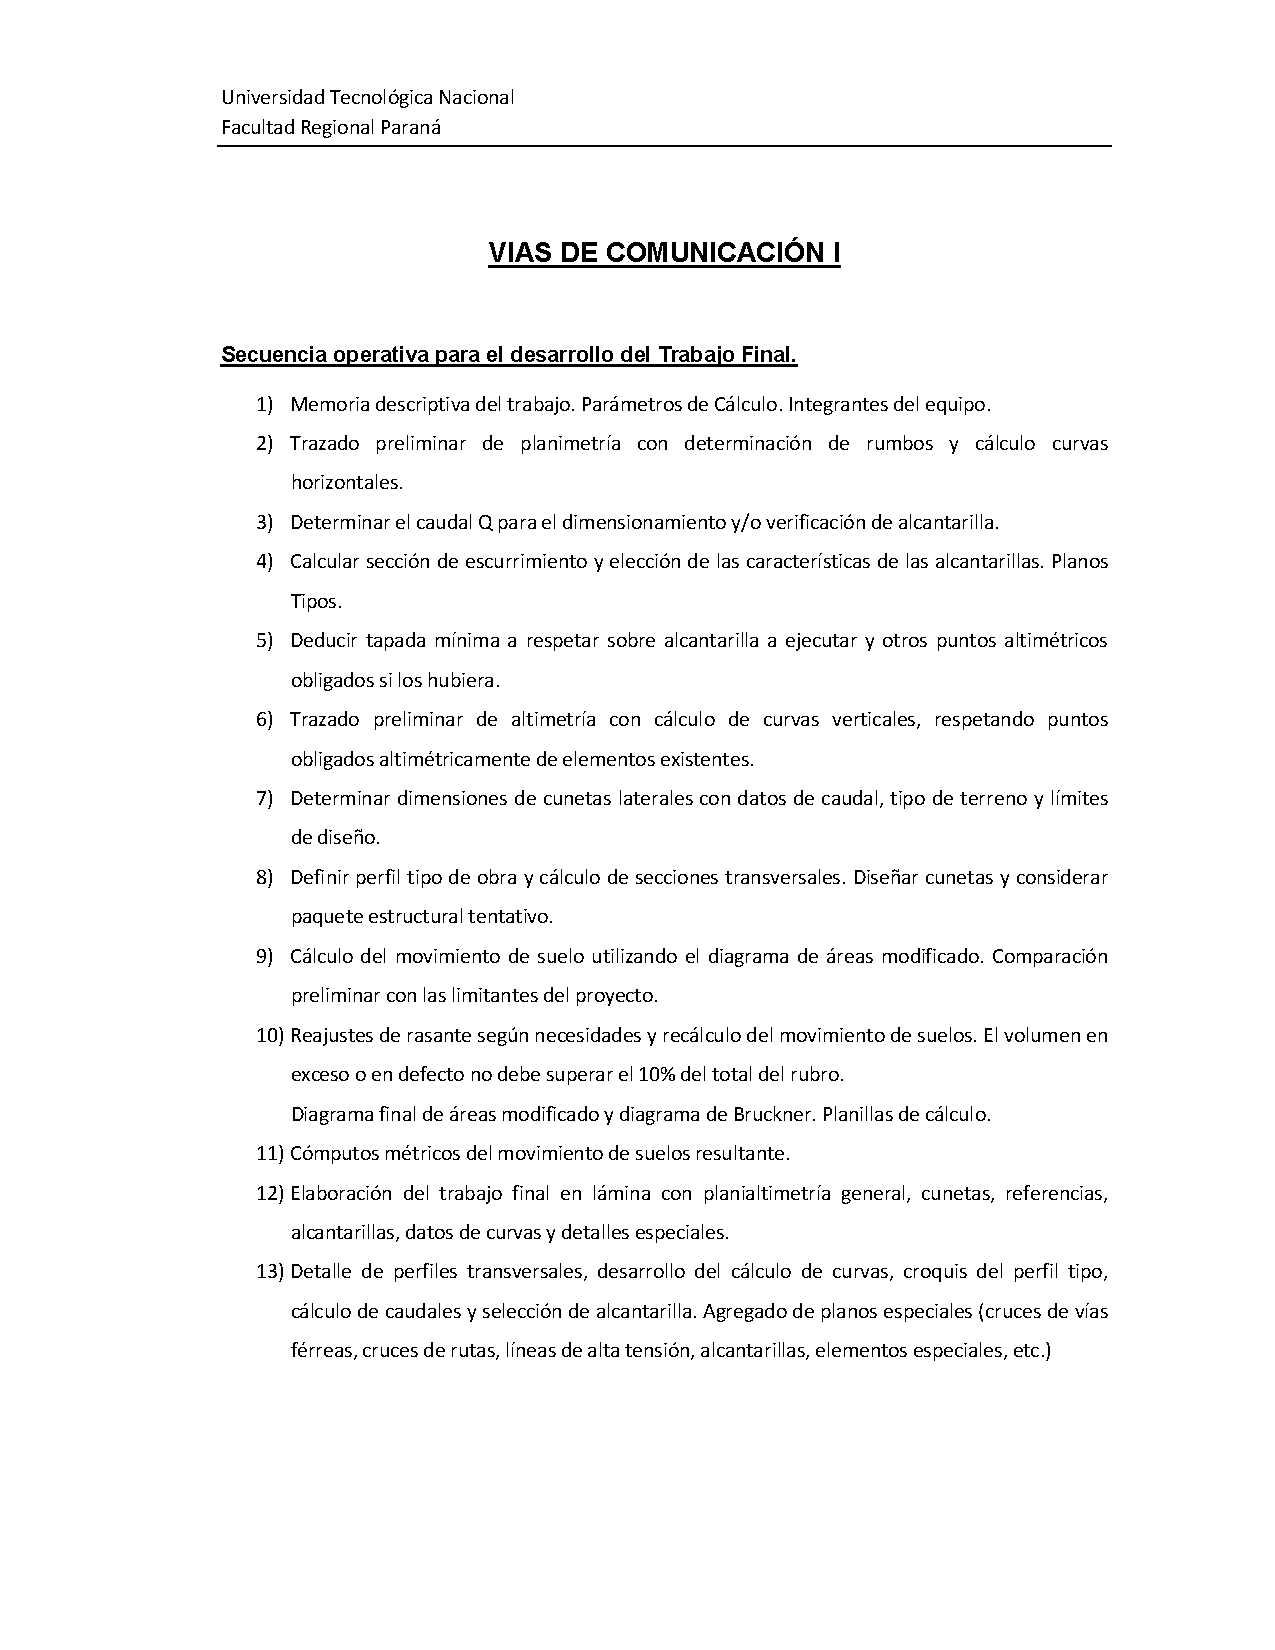
\includepdf[pages=-,addtotoc={
     1,section,1,Secuencia operativa,p1}]
     {consignas/Secuencia.pdf}       
            
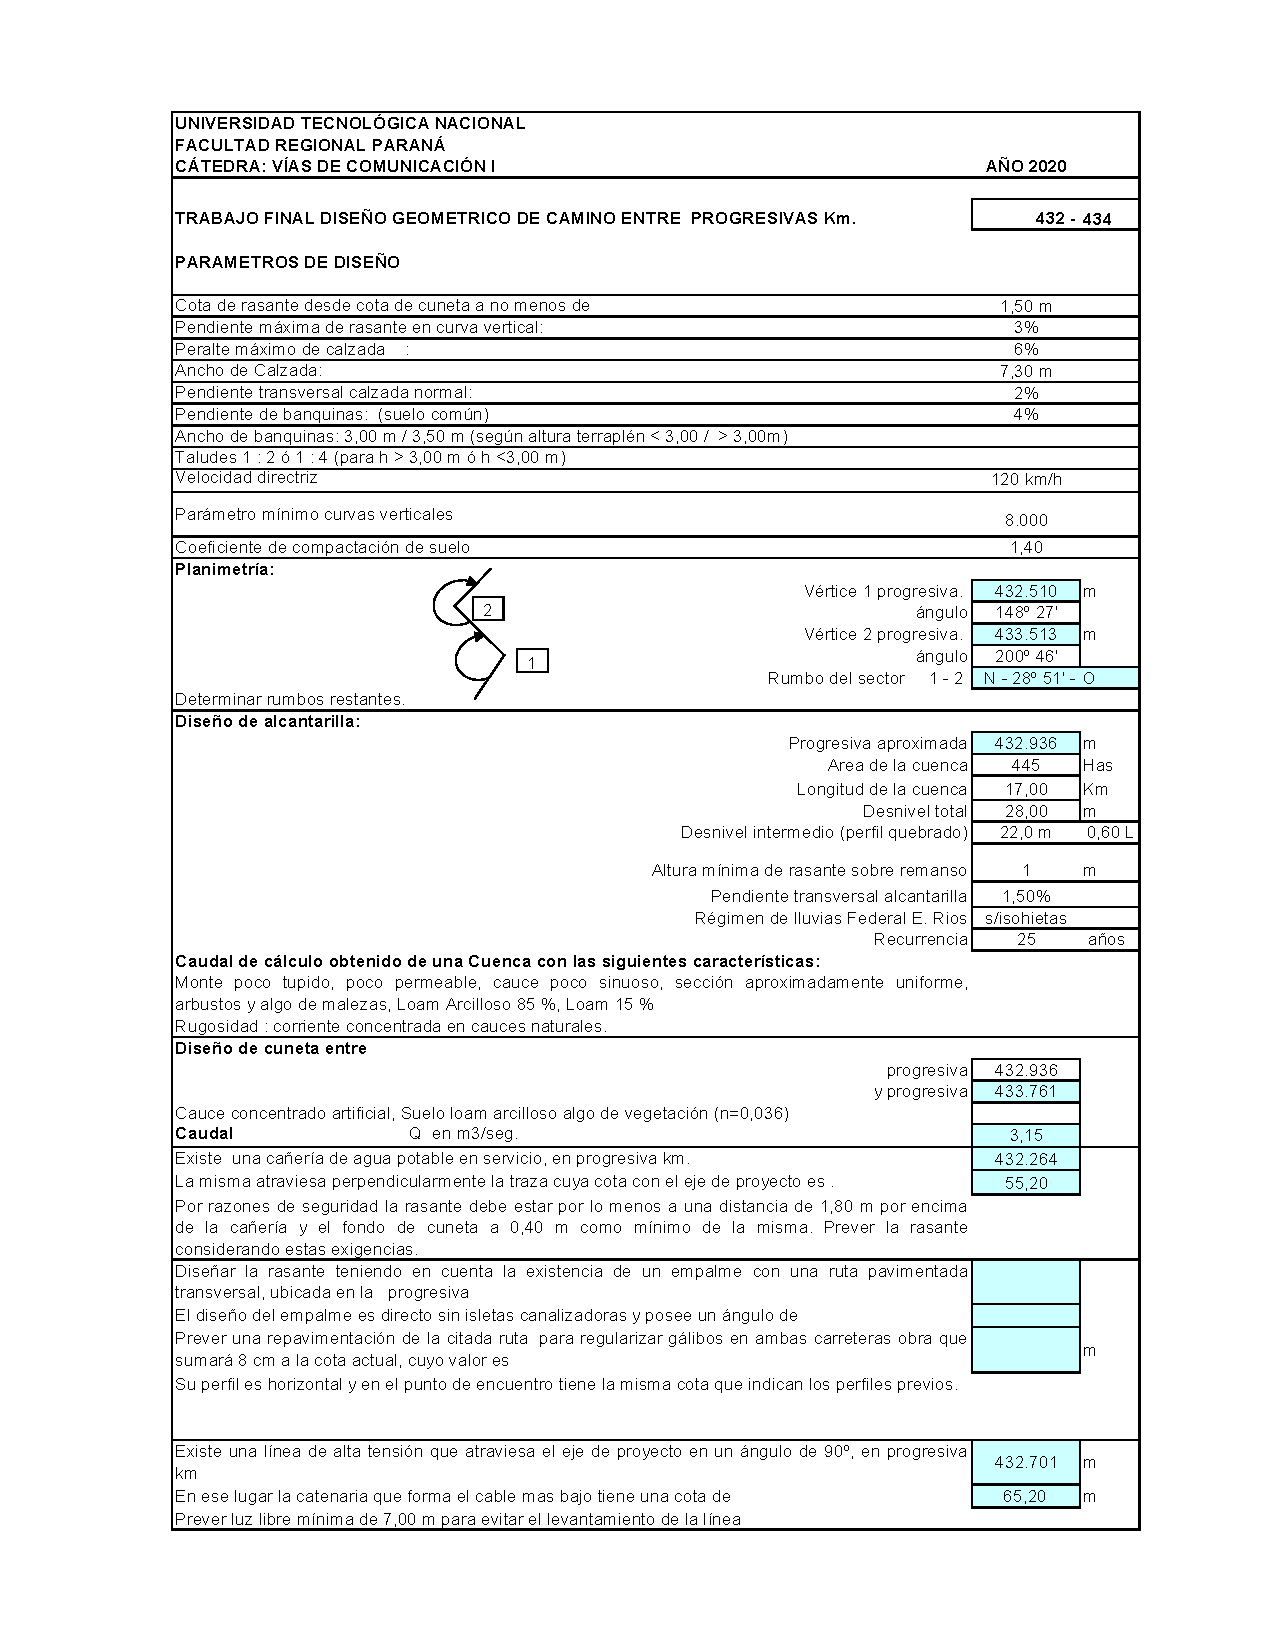
\includepdf[pages=-,addtotoc={
     1,section,1,Parametros de diseño,p2}]
     {consignas/parametros.pdf}
     
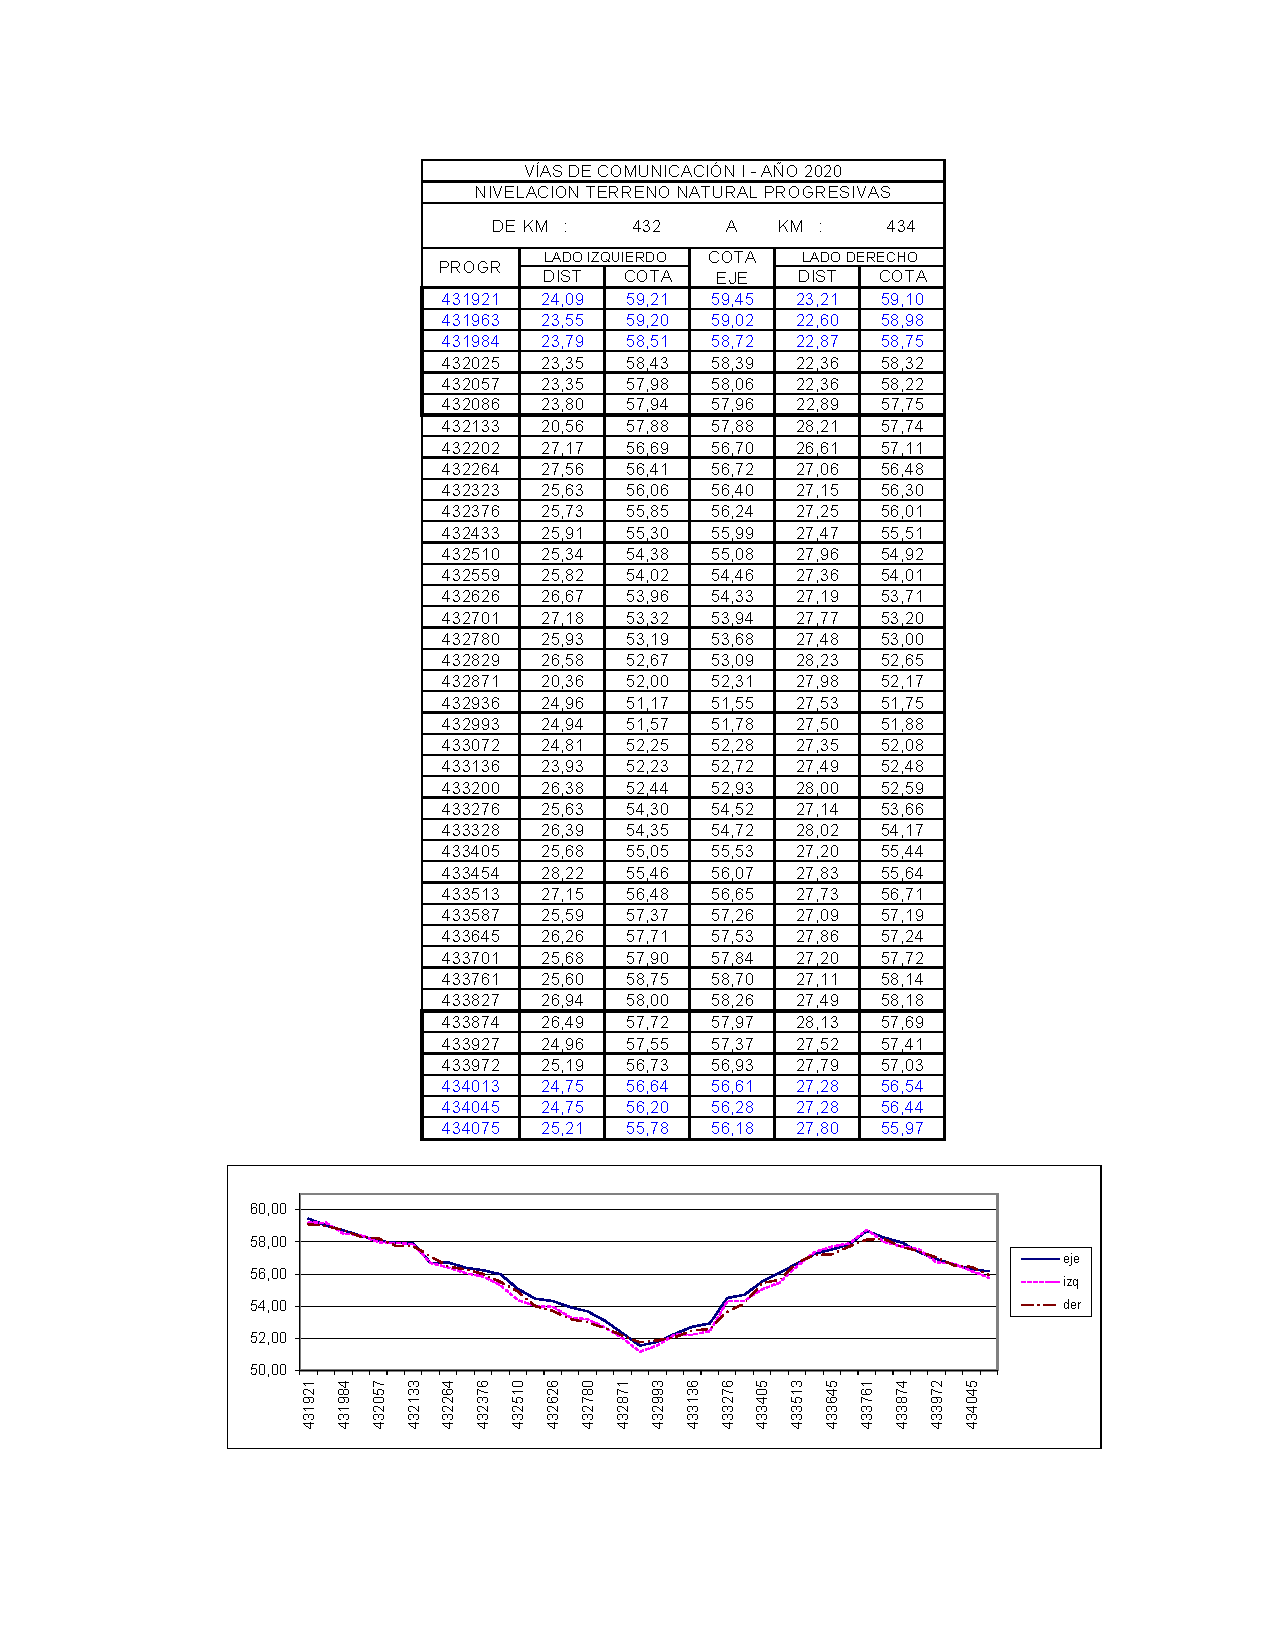
\includepdf[pages=-,addtotoc={
     1,section,1,Datos de nivelación,p3}]
     {consignas/nivelacion.pdf} 

\clearpage

\subfile{files/1-memoria}

\clearpage

\subfile{files/2-planimetria}
\subfile{files/3-alcantarilla}
\subfile{files/4-cunetas}
\subfile{files/5-altimetria}
\subfile{files/6-perfil-transversal}


\clearpage
\addcontentsline{toc}{section}{Bibliografía}
\printbibliography[title={Bibliografia}]

\end{document}
